% =====================================================================
%  FleetPulse - EC8203 Mini Project Final Technical Report
%  Author: P.S. Dilshan (EG/2020/3898)
%
%  How to compile: upload this whole folder (main.tex + figures/) to
%  https://www.overleaf.com (New Project -> Upload Project) and press Recompile.
%
%  Orange "To complete" boxes and [TBD] marks are filled in as the
%  remaining project phases are finished. Search for \tocomplete and \tbd
%  before submitting - none should remain.
% =====================================================================
\documentclass[11pt,a4paper]{article}

\usepackage[T1]{fontenc}
\usepackage[utf8]{inputenc}
\usepackage{lmodern}
\usepackage[a4paper,margin=2.5cm]{geometry}
\usepackage{amsmath}
\usepackage{graphicx}
\usepackage{booktabs}
\usepackage{tabularx}
\usepackage{array}
\usepackage{makecell}
\usepackage{xcolor}
\usepackage{float}
\usepackage{caption}
\usepackage{enumitem}
\usepackage{listings}
\usepackage[most]{tcolorbox}
\usepackage{tikz}
\usetikzlibrary{arrows.meta,positioning,fit,backgrounds}
\usepackage[hidelinks]{hyperref}

\captionsetup{font=small,labelfont=bf}
\setlist{nosep,leftmargin=*}
\renewcommand{\arraystretch}{1.25}
\newcolumntype{Y}{>{\raggedright\arraybackslash}X}

% ---------- helper macros ----------
% Inline code: \code{rt\_zone\_metrics}
\newcommand{\code}[1]{\texttt{\small #1}}
% Value not decided yet (version numbers of later phases etc.)
\newcommand{\tbd}{\textcolor{orange!80!black}{\textbf{[TBD]}}}
% Block that must be filled with real evidence before submission
\newcommand{\tocomplete}[1]{%
  \begin{tcolorbox}[colback=orange!6,colframe=orange!70!black,
    title=To complete (evidence from the running system),fonttitle=\bfseries\small,
    boxrule=0.6pt,arc=1mm]\small #1\end{tcolorbox}}
% Screenshot: shows the image if figures/<file> exists, otherwise a placeholder frame
\newcommand{\screenshot}[3]{%
  \begin{figure}[H]\centering
  \IfFileExists{figures/#1}%
    {\includegraphics[width=0.95\linewidth]{figures/#1}}%
    {\fbox{\parbox[c][4.5cm][c]{0.9\linewidth}{\centering\small\color{gray}
      Screenshot placeholder\\[2pt]\texttt{figures/#1}}}}%
  \caption{#2}\label{#3}\end{figure}}

\lstset{basicstyle=\ttfamily\footnotesize,breaklines=true,frame=single,
  backgroundcolor=\color{gray!6},rulecolor=\color{gray!40},columns=fullflexible}

% =====================================================================
\begin{document}

% ------------------------------------------------------------ title page
\begin{titlepage}
\centering
{\Large\bfseries University of Ruhuna\par}
\vspace{2pt}
{\large Faculty of Engineering\par}
\vspace{1.2cm}
\IfFileExists{figures/ruhuna_logo.png}{\includegraphics[width=3.4cm]{figures/ruhuna_logo.png}\par}{}
\vspace{1.2cm}
{\LARGE\bfseries FleetPulse: Ride-Hailing Fleet Operations Monitoring\par}
\vspace{0.4cm}
{\large A Lambda-Architecture Data Pipeline Using Kafka, Spark Structured Streaming,\\
Airflow and PostgreSQL\par}
\vspace{1.2cm}
{\large EC8203 -- Applied Big Data Engineering\par}
\vspace{4pt}
{\large Mini Project Assessment -- Final Technical Report\par}
\vspace{2cm}
{\large\bfseries Submitted by:\par}
\vspace{6pt}
{\large
\begin{tabular}{ll}
EG/2020/3898 & P.S. Dilshan \\
\end{tabular}\par}
\vspace{0.6cm}
{\normalsize Individual project (single-member team)\par}
\vfill
{\normalsize \tbd{} (submission date)\par}
\end{titlepage}

\tableofcontents
\newpage

% =====================================================================
\section*{Introduction}
\addcontentsline{toc}{section}{Introduction}

A ride-hailing operator has to answer two kinds of question about its fleet. Some are about
\emph{right now}: which areas are busy, how many vehicles are sitting idle, and how much the fleet
is earning at this moment. Others can only be answered \emph{after the fact}, once a day's costs
are known: which vehicles still make money after fuel and maintenance? This project builds a
prototype data platform called \textbf{FleetPulse} that answers both kinds of question for a
simulated fleet of 30 vehicles operating in five Colombo zones.

GPS and trip telemetry is streamed through Apache Kafka and processed continuously by Spark
Structured Streaming, which keeps live per-zone KPIs and raises an alert when a vehicle stays
idle too long. Once per simulated day, a CSV file of vehicle expenses arrives. An Apache Airflow
workflow then recomputes each vehicle's earnings from the raw event archive and joins them with
the expenses. The result is a per-vehicle profitability table and an HTML report. PostgreSQL
stores both views, and a FastAPI service combines them into a single answer per vehicle.
Structured logs, Prometheus metrics, alert rules and Grafana dashboards make the pipeline itself
observable.

The \textbf{Lambda architecture} was chosen because the two questions have different latency,
correctness and input characteristics. Live KPIs must be fresh but may be approximate, while the
daily profitability figures must be exact and reproducible. Section~\ref{sec:lambda} explains why
the alternative, Kappa, was rejected. All data is synthetic and time runs at an accelerated rate.
The system is a single-node academic prototype, not a production deployment.

% =====================================================================
\section{Use Case and Business Requirements}

\subsection{Selected use case}

This project implements \textbf{Use Case 1: Ride-Hailing Fleet Operations}. The business question
is:

\begin{quote}\itshape
What is fleet utilisation and earnings by area and time of day right now, and which vehicles are
becoming unprofitable once yesterday's fuel and maintenance costs are factored in?
\end{quote}

\noindent Two simulated sources feed the pipeline (Table~\ref{tab:sources}). A shared
configuration module (\code{common/fleet.py}) defines the zones, vehicle IDs and vehicle
profiles, so both sources describe the same fleet.

\begin{table}[H]
\centering\small
\begin{tabularx}{\linewidth}{l l Y l}
\toprule
\textbf{Source} & \textbf{Mode} & \textbf{Main fields} & \textbf{Volume} \\
\midrule
Vehicle telemetry & Stream (Kafka) &
\code{event\_id, trip\_id, driver\_id, vehicle\_id, lat, lon, speed, status, fare, zone,
timestamp, sim\_time, sim\_date} &
\makecell[l]{30 vehicles, 1 event\\per vehicle every 1--3 s\\($\approx$15 events/s)} \\
Vehicle expenses & Daily CSV file &
\code{vehicle\_id, fuel\_cost, maintenance\_cost, distance\_covered, service\_flag,
expense\_date} &
\makecell[l]{30 rows (+2 duplicates)\\per simulated day} \\
Fleet definition & Static config &
zones with bounding boxes, vehicle--driver assignment, vehicle profiles &
\makecell[l]{5 zones, 30 vehicles,\\25 drivers} \\
\bottomrule
\end{tabularx}
\caption{Input sources and their characteristics.}
\label{tab:sources}
\end{table}

The five zones are Fort, Kollupitiya, Bambalapitiya, Dehiwala and Nugegoda, each defined by a
latitude/longitude bounding box. Two groups of vehicles are given deliberate ``personalities'' so
that the business outputs are interesting rather than uniform:
\begin{itemize}
  \item \textbf{Lazy vehicles} (V007, V013, V021) wait 150--300 simulated minutes between rides.
    They should trigger idle alerts.
  \item \textbf{High-cost vehicles} (V004, V011, V019, V027) burn roughly twice as much fuel per km
    as a normal vehicle, and their maintenance cost grows by 20\% each simulated day. They should
    become unprofitable and show a falling-profit trend.
\end{itemize}

\subsection{Business requirements and interpretation}

Table~\ref{tab:req} breaks the business question down into requirements and maps each one to the
part of the system that addresses it.

\begin{table}[H]
\centering\small
\begin{tabularx}{\linewidth}{l Y Y}
\toprule
\textbf{ID} & \textbf{Requirement} & \textbf{Implementation} \\
\midrule
R1 & Show current utilisation and earnings by zone. &
Spark 1-minute tumbling windows per zone: active vehicles, idle ratio, trips per hour, earnings
(\code{rt\_zone\_metrics}). \\
R2 & Detect vehicles idling too long, promptly. &
Per-vehicle idle tracking in the speed layer; an alert opens once idle time exceeds a
configurable threshold (\code{idle\_alerts}). \\
R3 & Identify unprofitable vehicles using yesterday's costs. &
Airflow DAG joins the day's expenses with earnings recomputed from the Parquet lake
(\code{daily\_vehicle\_profitability}). \\
R4 & Detect vehicles trending towards unprofitability. &
A flag is set when a vehicle's profit has fallen on 2 or more consecutive simulated days. \\
R5 & Tolerate poor-quality data. &
Schema validation, range checks, a Kafka dead-letter topic, de-duplication by \code{event\_id},
watermarking, and cleaning of the CSV file. \\
R6 & Make results accessible. &
FastAPI endpoints for live zone data, idle alerts, the latest profitability report and a merged
per-vehicle view. \\
R7 & Make the pipeline observable. &
JSON logs, Prometheus metrics, four alert rules, two provisioned Grafana dashboards, and a
\code{/health} endpoint. \\
R8 & Be reproducible and testable. &
Docker Compose, a single \code{.env} configuration file, deterministic expense data, unit tests
and a demo script. \\
\bottomrule
\end{tabularx}
\caption{Requirements derived from the business question.}
\label{tab:req}
\end{table}

\subsection{Simulation assumptions}

\paragraph{Accelerated time.} One simulated day lasts \code{SIM\_DAY\_SECONDS}~$=600$ real
seconds, so time runs $86\,400/600 = 144\times$ faster than reality: one real minute equals 2.4
simulated hours. Every component converts real time to simulated time with the same formula,
\[
  t_{\text{sim}} = \text{SIM\_START\_DATE} + (t_{\text{real}} - t_{\text{anchor}})\times 144,
\]
where $t_{\text{anchor}}$ is written once to a shared file by whichever component starts first.
This keeps every container in agreement about the current simulated day.

\paragraph{Two timestamps per event.} Each event carries its real \code{timestamp}, which Spark
uses for windows and watermarks, and its simulated \code{sim\_time}/\code{sim\_date}, which are
used for lake partitioning and the daily batch. Windows are defined in real time on purpose. With
one event per vehicle every 1--3 real seconds, a 1-minute window holds 20--60 readings per
vehicle, so the window aggregates are meaningful rather than single readings.

\paragraph{Trip and fare model.} Each vehicle cycles through
\code{idle}~$\rightarrow$~\code{enroute}~$\rightarrow$~\code{on\_trip}~$\rightarrow$~\code{idle}.
Idle waits are exponentially distributed: shorter during the morning and evening rush (simulated
07:00--09:59 and 17:00--19:59) and longer at night. When a trip ends, the vehicle emits one event
with $\text{fare} = 150 + 95\times\text{km}$~LKR, plus a 20\% surge at rush hour. Every other
event has $\text{fare}=0$, so downstream $\text{trips} = \text{count}(\text{fare}>0)$ and
$\text{earnings} = \sum\text{fare}$.

\paragraph{Daily expenses.} At the start of simulated day $D$, the expense producer writes
\code{expenses\_$\langle D{-}1\rangle$.csv}: yesterday's costs, matching the business wording.
The values are seeded by (vehicle, date), so regenerating a file gives identical numbers.

\paragraph{Fault injection.} About 2\% of telemetry events are followed by a corrupted copy
(null \code{vehicle\_id}, impossible coordinates or a negative fare), and about 1\% are sent twice
with the same \code{event\_id}. Each expense file contains two duplicate rows and one blank
\code{fuel\_cost}. The faults are added alongside the clean data, never in place of it, so the
correct results remain known.

% =====================================================================
\section{Architecture Decision: Lambda versus Kappa}
\label{sec:lambda}

\subsection{Decision and justification}

The selected architecture is \textbf{Lambda}. A \emph{speed layer} (Spark Structured Streaming)
keeps an approximate, low-latency view of the fleet. A \emph{batch layer} (Airflow) recomputes an
exact daily view from an immutable master dataset, the raw Parquet lake. A \emph{serving layer}
(FastAPI) combines the two.

\begin{table}[H]
\centering\small
\begin{tabularx}{\linewidth}{l Y Y}
\toprule
\textbf{Criterion} & \textbf{Lambda (selected)} & \textbf{Kappa (considered, rejected)} \\
\midrule
Input shape & Handles a continuous stream and a once-a-day file naturally, each in its own
layer. & The daily expense CSV would have to be replayed into Kafka as events just to fit the
model. \\
Correctness & Daily earnings are recomputed from the raw lake. Duplicates, late events and replayed
micro-batches cannot distort the profitability figures. & Correctness depends on the streaming
job's state; fixing a bug means replaying the whole topic. \\
Re-running a day & An Airflow run for one \code{sim\_date} rebuilds that day's rows
idempotently. & Needs a full replay from Kafka, which requires long topic retention. \\
Orchestration & Airflow's file sensor, retries and run history match the ``wait for file, then
process'' workflow. & Kafka itself has no notion of ``today's file has arrived''; this logic
would have to be custom-built. \\
Cost & Two code paths (earnings are computed twice) and more services to run. & One code path and
simpler operations. \\
\bottomrule
\end{tabularx}
\caption{Architecture options evaluated against this use case.}
\label{tab:lambda}
\end{table}

Kappa was rejected for three reasons specific to this use case:
\begin{enumerate}
  \item \textbf{The cost data is genuinely batch.} One small file arrives per day. Turning it into a
    stream adds machinery without any latency benefit, because profitability cannot be known before
    the costs arrive.
  \item \textbf{Profitability must be exact and auditable.} The speed layer is deliberately
    approximate: \code{approx\_count\_distinct}, a 2-minute watermark that drops very late events,
    and at-least-once \code{foreachBatch} writes. The batch layer corrects this by recomputing from
    the lake and de-duplicating on \code{event\_id}.
  \item \textbf{The single-broker Kafka is not a durable log.} With replication factor 1 and
    24-hour retention, Kafka cannot serve as the long-term source of truth that Kappa requires.
    The Parquet lake serves that role instead.
\end{enumerate}

The price of Lambda is that earnings logic exists in two places: the Spark window aggregation and
the batch recomputation. Both use the same definition ($\text{trips}=\text{count}(\text{fare}>0)$,
$\text{earnings}=\sum\text{fare}$) and the same shared configuration module, which limits drift
between them. Kappa would become attractive if expenses arrived as a continuous stream (for
example from fuel-card transactions) and Kafka were run as a replicated, long-retention log.

% =====================================================================
\section{Designed System Architecture}

Figure~\ref{fig:arch} shows the full pipeline. Solid arrows are data flow and dashed arrows are
monitoring. Every component runs as a container in one Docker Compose project.

\begin{figure}[H]
\centering
\resizebox{\linewidth}{!}{%
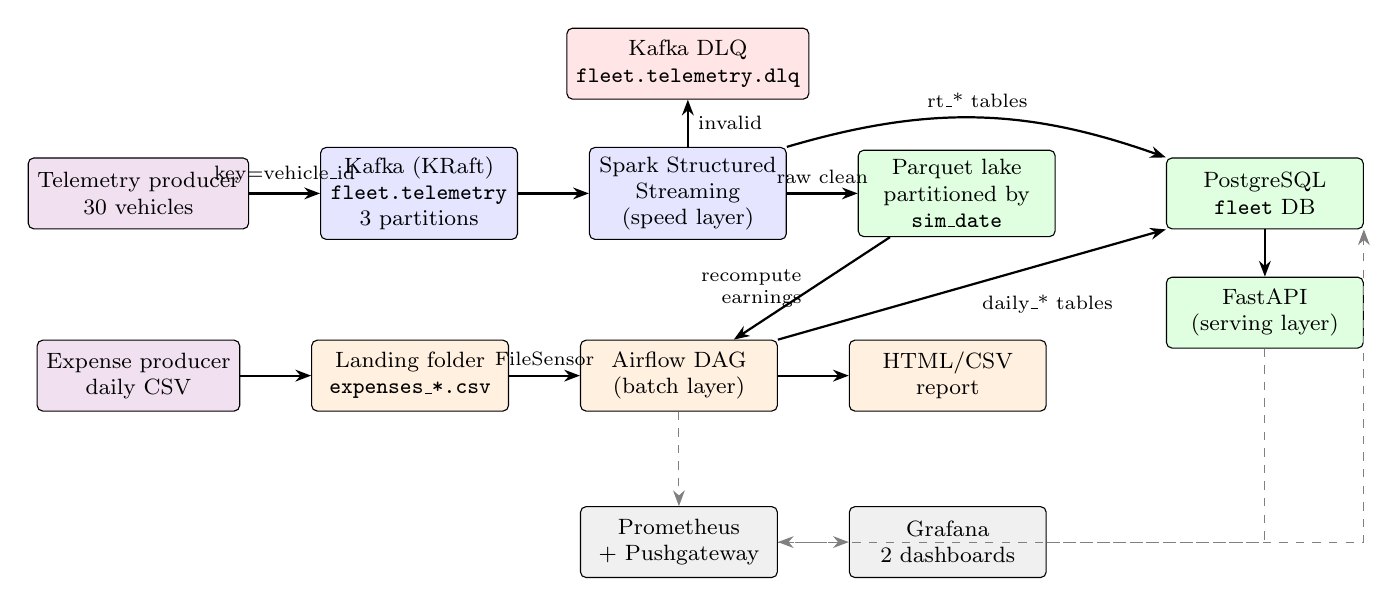
\begin{tikzpicture}[
  node distance=6mm and 9mm,
  box/.style={draw,rounded corners=2pt,align=center,font=\footnotesize,minimum height=9mm,
              minimum width=25mm,fill=#1},
  box/.default=white,
  flow/.style={-{Stealth[length=2mm]},thick},
  mon/.style={-{Stealth[length=2mm]},dashed,gray}]
  % speed path
  \node[box=violet!12] (tp) {Telemetry producer\\30 vehicles};
  \node[box=blue!10, right=of tp] (kafka) {Kafka (KRaft)\\\texttt{fleet.telemetry}\\3 partitions};
  \node[box=blue!10, right=of kafka] (spark) {Spark Structured\\Streaming\\(speed layer)};
  \node[box=red!10, above=of spark] (dlq) {Kafka DLQ\\\texttt{fleet.telemetry.dlq}};
  \node[box=green!12, right=of spark] (lake) {Parquet lake\\partitioned by\\\texttt{sim\_date}};
  % batch path
  \node[box=violet!12, below=14mm of tp] (ep) {Expense producer\\daily CSV};
  \node[box=orange!12, right=of ep] (land) {Landing folder\\\texttt{expenses\_*.csv}};
  \node[box=orange!12, right=of land] (air) {Airflow DAG\\(batch layer)};
  \node[box=orange!12, right=of air] (rep) {HTML/CSV\\report};
  % serving
  \node[box=green!12, right=14mm of lake] (pg) {PostgreSQL\\\texttt{fleet} DB};
  \node[box=green!12, below=of pg] (api) {FastAPI\\(serving layer)};
  % monitoring
  \node[box=gray!12, below=12mm of air] (prom) {Prometheus\\+ Pushgateway};
  \node[box=gray!12, right=of prom] (graf) {Grafana\\2 dashboards};

  \draw[flow] (tp) -- node[above,font=\scriptsize]{key=vehicle\_id} (kafka);
  \draw[flow] (kafka) -- (spark);
  \draw[flow] (spark) -- node[right,font=\scriptsize]{invalid} (dlq);
  \draw[flow] (spark) -- node[above,font=\scriptsize]{raw clean} (lake);
  \draw[flow] (spark.north east) to[bend left=18] node[above,font=\scriptsize]{rt\_* tables} (pg.north west);
  \draw[flow] (ep) -- (land);
  \draw[flow] (land) -- node[above,font=\scriptsize]{FileSensor} (air);
  \draw[flow] (lake) -- node[left,font=\scriptsize,align=right]{recompute\\earnings} (air);
  \draw[flow] (air) -- (rep);
  \draw[flow] (air.north east) -- node[below right,font=\scriptsize]{daily\_* tables} (pg.south west);
  \draw[flow] (pg) -- (api);
  \draw[mon] (prom) -- (graf);
  \draw[mon] (graf.east) -| (pg.south east);
  \draw[mon] (air) -- (prom);
  \draw[mon] (api.south) |- (prom.east);
\end{tikzpicture}}
\caption{FleetPulse Lambda architecture: speed layer (top), batch layer (middle), serving and
monitoring (right and bottom).}
\label{fig:arch}
\end{figure}

\subsection{Ingestion}

The telemetry producer publishes JSON events to the \code{fleet.telemetry} topic, which has three
partitions. Each message is keyed by \code{vehicle\_id}. Kafka hashes the key to choose a
partition, so all events of one vehicle land in the same partition in order, while up to three
consumers can read in parallel. The producer uses \code{acks=all} and
\code{enable.idempotence=true}: a message only counts as sent once the broker has stored it, and a
retry can never write it twice. The producer waits for Kafka with exponential backoff before
starting. On \code{SIGINT}/\code{SIGTERM} it flushes its buffer before exiting.

The expense producer writes each CSV to a hidden \code{.tmp} file and then renames it to its final
name. The rename is atomic, so the Airflow file sensor never sees a half-written file.

\subsection{Speed layer}

A single Spark application runs three streaming queries over one parsed and validated input:
\begin{enumerate}
  \item \textbf{dlq}: records that fail validation are written to \code{fleet.telemetry.dlq}
    together with the reason, the original payload, and their Kafka partition and offset.
  \item \textbf{clean\_events}: valid events pass through a 2-minute watermark and
    \code{dropDuplicatesWithinWatermark(event\_id)}. A \code{foreachBatch} sink then
    (a)~appends them to the Parquet lake, (b)~updates the latest state of each vehicle in
    \code{rt\_vehicle\_status}, and (c)~opens or resolves rows in \code{idle\_alerts}.
  \item \textbf{zone\_metrics}: 1-minute tumbling windows per zone in \code{update} output mode,
    upserted into \code{rt\_zone\_metrics}, so dashboards see each window fill up live.
\end{enumerate}
Each query has its own checkpoint directory. If the job crashes, Docker restarts the container and
Spark resumes from the last committed micro-batch.

\subsection{Batch layer}

The Airflow DAG \code{daily\_fleet\_reconciliation} runs once per simulated day
(Figure~\ref{fig:dag}). The key design decision is that daily earnings are \textbf{recomputed from
the raw Parquet lake}, not copied from the speed layer's tables. The lake is the master dataset,
and recomputing from it, with de-duplication on \code{event\_id}, corrects anything the speed layer
approximated or double-counted.

\begin{figure}[H]
\centering
\resizebox{\linewidth}{!}{%
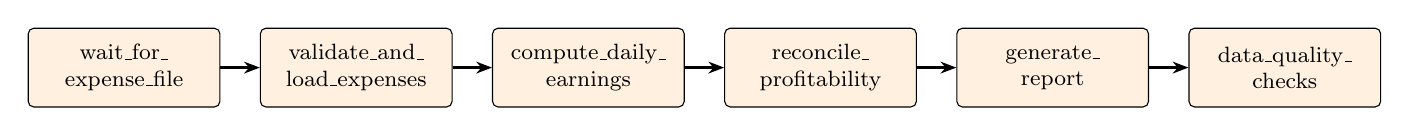
\begin{tikzpicture}[node distance=5mm,
  t/.style={draw,rounded corners=2pt,fill=orange!12,align=center,font=\footnotesize,
            minimum height=10mm,text width=22mm},
  a/.style={-{Stealth[length=2mm]},thick}]
  \node[t] (s) {wait\_for\_\\expense\_file};
  \node[t,right=of s] (v) {validate\_and\_\\load\_expenses};
  \node[t,right=of v] (e) {compute\_daily\_\\earnings};
  \node[t,right=of e] (r) {reconcile\_\\profitability};
  \node[t,right=of r] (g) {generate\_\\report};
  \node[t,right=of g] (q) {data\_quality\_\\checks};
  \foreach \x/\y in {s/v,v/e,e/r,r/g,g/q} \draw[a] (\x) -- (\y);
\end{tikzpicture}}
\caption{Airflow DAG \code{daily\_fleet\_reconciliation}.}
\label{fig:dag}
\end{figure}

\tocomplete{Confirm the final DAG structure (Phase 4): sensor type and timeout, retry settings,
how the logical date maps to the simulated date, and whether earnings are computed with pandas or
PySpark.}

\subsection{Storage and serving}

PostgreSQL 16 hosts two separate databases: \code{fleet} for business data and \code{airflow} for
Airflow's metadata, so resetting one never affects the other. Tables prefixed \code{rt\_} belong to
the speed layer and tables prefixed \code{daily\_} to the batch layer. Every table has a primary
key and every write is an upsert (\code{INSERT \ldots{} ON CONFLICT DO UPDATE}), so re-running a
micro-batch or a DAG run overwrites rows instead of duplicating them.

The FastAPI service combines the two layers. \code{GET /vehicles/\{vehicle\_id\}/status}, for
example, returns a vehicle's latest real-time state alongside its most recent profitability row.

% =====================================================================
\section{Technology Stack and Rationale}

\begin{table}[H]
\centering\small
\begin{tabularx}{\linewidth}{l l Y}
\toprule
\textbf{Concern} & \textbf{Technology} & \textbf{Why it fits this use case / alternatives} \\
\midrule
Ingestion & Apache Kafka 3.8.0 (KRaft) &
Buffers telemetry and decouples the producer from the consumers. Keying by vehicle preserves
per-vehicle order. KRaft removes ZooKeeper, saving memory on a laptop. A direct database insert
from the producer was rejected because it ties the sources to storage and leaves nothing to
replay. \\
Stream processing & Spark Structured Streaming 3.5.3 &
Built-in event-time windows, watermarks, de-duplication, checkpointing and a Kafka connector.
\emph{Apache Storm} offers lower per-event latency, but it has no built-in event-time windowing
or exactly-once state, and sub-second latency is unnecessary here. \\
Batch orchestration & Apache Airflow \tbd{} (LocalExecutor) &
FileSensor, retries, run history and per-date reruns match the daily-file workflow. Plain cron
offers none of these. LocalExecutor avoids running Celery and Redis. \\
Batch processing & \tbd{} (pandas / PySpark) &
A day is about 15\,000 events and 30 expense rows, which fits comfortably on one node. \\
Serving store & PostgreSQL 16.4 &
Relational joins between the speed and batch tables, upserts and indexed date queries.
\emph{Cassandra} handles massive write throughput, but this workload needs joins and ad-hoc
reporting, not distributed writes. \\
Master dataset & Parquet on local disk &
Columnar and compressed, and partitioned by \code{sim\_date}, so the batch job reads only one day.
\emph{HDFS} would add a NameNode and DataNodes for no benefit at this scale; in production the
same layout would move to object storage (S3, GCS or ADLS). \\
Serving API & FastAPI \tbd{} &
Typed responses and automatically generated OpenAPI/Swagger documentation. \\
Observability & Prometheus \tbd{}, Grafana \tbd{} &
Pull-based metrics for long-running services, Pushgateway for short-lived Airflow tasks, and
dashboards and datasources provisioned from files. \\
Packaging & Docker Compose &
One command starts the whole stack, and image versions are pinned. \\
\bottomrule
\end{tabularx}
\caption{Technology choices and rationale.}
\label{tab:stack}
\end{table}

% =====================================================================
\section{Implementation Details}

\subsection{Data quality rules (speed layer)}

Messages are parsed with an \emph{explicit} schema. Each record receives an \code{error\_reason}
column: the first rule it breaks, or \code{NULL} if it is valid (Table~\ref{tab:dq}). Null checks
come first, because in SQL a comparison such as \code{NULL < 0} is neither true nor false and would
otherwise let a bad record through. All rules are native Spark expressions rather than Python
UDFs, so they run inside the JVM.

\begin{table}[H]
\centering\small
\begin{tabularx}{\linewidth}{l Y}
\toprule
\textbf{\code{error\_reason}} & \textbf{Condition} \\
\midrule
\code{malformed\_json} & JSON could not be parsed (no \code{event\_id}). \\
\code{null\_vehicle\_id} & \code{vehicle\_id} is null or blank. \\
\code{missing\_timestamp} & \code{timestamp} is null or unparseable. \\
\code{impossible\_coordinates} & lat/lon is null or outside greater Colombo (lat 6.80--7.00,
lon 79.80--79.95). \\
\code{negative\_fare} & \code{fare} is null or $<0$. \\
\code{invalid\_speed} & \code{speed} is null or $<0$. \\
\code{invalid\_status} & \code{status} is not one of \code{idle}, \code{enroute},
\code{on\_trip}. \\
\code{unknown\_zone} & \code{zone} is not one of the five configured zones. \\
\midrule
\textit{duplicate} & Same \code{event\_id} seen within the watermark: silently dropped. \\
\bottomrule
\end{tabularx}
\caption{Validation rules applied to every telemetry message.}
\label{tab:dq}
\end{table}

\subsection{Real-time KPIs and idle alerts}

For each 1-minute window and zone, the speed layer computes:
\begin{itemize}
  \item \textbf{active vehicles}: distinct vehicles seen, using \code{approx\_count\_distinct},
    which works in streaming and is effectively exact at this cardinality;
  \item \textbf{idle ratio}: idle pings divided by all pings, i.e.\ the share of time vehicles
    spent idle;
  \item \textbf{trips per hour}: completed trips divided by the window length in
    \emph{simulated} hours ($60\,\text{s}\times144/3600 = 2.4$ simulated hours);
  \item \textbf{earnings}: the sum of fares completed in the window, credited to the pickup zone.
\end{itemize}

\paragraph{Idle alert rule.} For each vehicle, the start of its current idle period
(\code{idle\_since}) is tracked across micro-batches. A non-idle event clears it, and consecutive
idle events keep the original start time, even if the idle period began in an earlier batch. An
alert opens when
\[
  \text{event\_time} - \text{idle\_since} > \text{IDLE\_ALERT\_SIM\_MINUTES}
  \;(90\ \text{sim-min} = 37.5\ \text{real s}).
\]
A partial unique index (\code{UNIQUE (vehicle\_id) WHERE status='open'}) guarantees at most one
open alert per vehicle. The alert is resolved automatically when the vehicle moves again. Idle time
is measured in \emph{event time}, so replaying old data gives the same alerts.

\subsection{Profitability calculation (batch layer)}

For vehicle $v$ on simulated day $d$:
\begin{align*}
  \text{earnings}_{v,d} &= \textstyle\sum \text{fare} \quad\text{over de-duplicated lake events with fare}>0\\
  \text{total\_cost}_{v,d} &= \text{fuel\_cost}_{v,d} + \text{maintenance\_cost}_{v,d}\\
  \text{profit}_{v,d} &= \text{earnings}_{v,d} - \text{total\_cost}_{v,d}\\
  \text{margin}_{v,d} &= \text{profit}_{v,d} / \text{earnings}_{v,d}
     \quad(\text{undefined if earnings}=0)\\
  \text{cost\_per\_km}_{v,d} &= \text{total\_cost}_{v,d} / \text{distance\_covered}_{v,d}
\end{align*}
A vehicle is flagged \textbf{unprofitable} if $\text{profit}<0$ or
$\text{margin}<\text{UNPROFITABLE\_MARGIN\_THRESHOLD}$ (default 0.10). It is flagged
\textbf{trending unprofitable} if its profit has fallen on two or more consecutive simulated days.

\tocomplete{Phase 4: describe how the blank \code{fuel\_cost} row is handled (dropped or
imputed), how duplicates are removed, and any data-quality checks the final task performs.}

\subsection{Data model}

\begin{table}[H]
\centering\small
\begin{tabularx}{\linewidth}{l l l Y}
\toprule
\textbf{Table} & \textbf{Layer} & \textbf{Primary key} & \textbf{Content} \\
\midrule
\code{rt\_zone\_metrics} & Speed & (window\_start, zone) & Per-window zone KPIs. \\
\code{rt\_vehicle\_status} & Speed & vehicle\_id & Latest state of each vehicle, including
\code{idle\_since}. \\
\code{idle\_alerts} & Speed & alert\_id & Alert history; at most one open alert per vehicle. \\
\code{vehicle\_expenses} & Batch & (vehicle\_id, expense\_date) & Cleaned expense rows. \\
\code{daily\_vehicle\_earnings} & Batch & (vehicle\_id, sim\_date) & Earnings recomputed from the
lake. \\
\code{daily\_vehicle\_profitability} & Batch & (vehicle\_id, sim\_date) & Profit, margin,
cost/km and both unprofitability flags. \\
\code{batch\_run\_log} & Batch & run\_id & Audit trail of task runs and DQ results. \\
\bottomrule
\end{tabularx}
\caption{PostgreSQL tables in the \code{fleet} database.}
\label{tab:model}
\end{table}

\subsection{Serving API}

\begin{table}[H]
\centering\small
\begin{tabularx}{\linewidth}{l Y}
\toprule
\textbf{Endpoint} & \textbf{Returns} \\
\midrule
\code{GET /health} & \code{healthy}/\code{degraded}/\code{unhealthy}, with checks of Kafka,
Postgres and data freshness. \\
\code{GET /metrics} & Prometheus metrics (request count and latency). \\
\code{GET /fleet/realtime} & Latest window per zone: active vehicles, idle ratio, trips/hour,
earnings. \\
\code{GET /fleet/realtime/zones/\{zone\}} & Recent windows for one zone. \\
\code{GET /alerts/idle} & Currently open idle alerts. \\
\code{GET /reports/profitability/latest} & The most recent batch profitability results. \\
\code{GET /vehicles/\{vehicle\_id\}/status} & \textbf{Merged view}: real-time state plus latest
profitability. \\
\bottomrule
\end{tabularx}
\caption{FastAPI endpoints (Phase 5).}
\label{tab:api}
\end{table}

% =====================================================================
\section{Observability Design}

Observability is designed around four questions: \emph{Is data still arriving? Is input quality
getting worse? Did the daily job run? Is the fleet behaving abnormally?} Metrics answer these
questions, alert rules flag them, and structured logs explain why.

\subsection{Structured logging}

Every service writes one JSON object per line with the same core fields, so logs can be filtered
and counted by field rather than parsed as free text:

\begin{lstlisting}
{"timestamp": "2026-11-16T08:46:20.918+00:00", "level": "INFO",
 "service": "telemetry-producer", "stage": "ingestion", "event": "producer_progress",
 "message": "Producer progress", "record_count": 141, "sim_date": "2025-01-01",
 "sim_time": "00:24", "idle": 13, "enroute": 6, "on_trip": 11}
\end{lstlisting}

\noindent \code{stage} is one of \code{ingestion}, \code{processing}, \code{storage} or
\code{serving}. Context fields such as \code{vehicle\_id}, \code{sim\_date}, \code{batch\_id} and
\code{record\_count} are added where relevant.

\subsection{Metrics}

\begin{table}[H]
\centering\small
\begin{tabularx}{\linewidth}{l l Y}
\toprule
\textbf{Metric} & \textbf{Source} & \textbf{Why it matters} \\
\midrule
\code{events\_produced\_total} & producer & Throughput; confirms the source is alive. \\
\code{events\_failed\_total} & producer & Kafka delivery failures. \\
\code{invalid\_events\_injected\_total\{reason\}} & producer & Ground truth for validating the
DLQ count. \\
\code{stream\_batches\_processed\_total\{query\}} & Spark & Confirms each query is making
progress. \\
\code{stream\_records\_processed\_total} & Spark & Valid records processed. \\
\code{stream\_records\_dlq\_total\{reason\}} & Spark & Data-quality signal for the error-rate
alert. \\
\code{stream\_batch\_duration\_seconds} & Spark & Detects a job falling behind its 10\,s
trigger. \\
\code{last\_event\_timestamp} & Spark & Freshness; a running job can still be stalled. \\
\code{batch\_runs\_total\{status\}} & Airflow (Pushgateway) & Detects failed daily runs. \\
\code{batch\_records\_loaded\_total} & Airflow (Pushgateway) & Volume loaded per run. \\
\code{batch\_duration\_seconds} & Airflow (Pushgateway) & Detects slow runs. \\
API request count and latency & FastAPI & Serving-layer health. \\
\bottomrule
\end{tabularx}
\caption{Prometheus metrics. Long-running services are scraped; short-lived Airflow tasks push
to a Pushgateway.}
\label{tab:metrics}
\end{table}

\subsection{Alert rules and dashboards}

\begin{table}[H]
\centering\small
\begin{tabularx}{\linewidth}{l Y Y}
\toprule
\textbf{Alert} & \textbf{Condition} & \textbf{Failure it catches} \\
\midrule
NoDataReceived & \code{time() - last\_event\_timestamp > 120} & Producer down, Kafka down, or
Spark stalled. \\
HighDLQRate & DLQ records / all records $>5\%$ & Upstream schema change or broken sensor
data. \\
BatchJobFailed & failed run, or no expense file for the simulated day & Missing daily costs,
which means profitability cannot be trusted. \\
VehicleIdleTooLong & open idle alert exists & Business alert: a vehicle is wasting capacity. \\
\bottomrule
\end{tabularx}
\caption{Alert rules (Phase 6).}
\label{tab:alerts}
\end{table}

Two Grafana dashboards are provisioned from files, so they appear straight after
\code{docker compose up}: \textbf{Fleet Operations} (business KPIs from PostgreSQL) and
\textbf{Pipeline Health} (throughput, DLQ rate, freshness and batch status from Prometheus).

\tocomplete{Phase 6: final PromQL expressions, \code{for:} durations, and Grafana panel list.}

% =====================================================================
\section{Results and Evaluation}

\subsection{Ingestion results}

The following results were measured on the running system on 16~November~2026, in the first
$\approx$30 seconds after a clean start (simulated day 2025-01-01).

\begin{table}[H]
\centering\small
\begin{tabular}{l r}
\toprule
\textbf{Measurement} & \textbf{Value} \\
\midrule
Messages per partition of \code{fleet.telemetry} (P0 / P1 / P2) & 100 / 175 / 211 \\
Events acknowledged by Kafka (\code{events\_produced\_total}) & 1\,634 \\
Delivery failures (\code{events\_failed\_total}) & 0 \\
Corrupted records injected (null id / bad coordinates / negative fare) & 12 / 6 / 12 \\
Duplicate events injected & 17 \\
Non-null keys mapped to more than one partition & 0 \\
Events left undelivered after \code{docker stop} (graceful shutdown) & 0 \\
\bottomrule
\end{tabular}
\caption{Ingestion-layer measurements.}
\label{tab:ingest}
\end{table}

All three partitions received data, and every vehicle's events stayed in a single partition.
The only key that appeared in several partitions was \code{null}, from deliberately corrupted
records, which is expected because Kafka spreads null-key messages across partitions. A test
expense file contained 32 rows (30 vehicles plus 2 duplicates) and exactly one blank
\code{fuel\_cost}. The high-cost vehicles' daily costs were about three times those of a normal
vehicle.

\subsection{Speed-layer results}
\tocomplete{Phase 3: sample rows from \code{rt\_zone\_metrics} (per zone: active vehicles, idle
ratio, trips/hour, earnings); DLQ count compared with \code{invalid\_events\_injected\_total};
duplicate count removed; idle alerts raised for V007, V013 and V021 (\code{SELECT} from
\code{idle\_alerts}); Parquet lake file and partition listing.}

\subsection{Batch-layer results}
\tocomplete{Phase 4: profitability table for one simulated day (vehicle, trips, earnings, costs,
profit, margin, flags). Explicitly show that V004, V011, V019 and V027 are flagged unprofitable
and/or trending. Show the speed-layer vs batch-layer earnings comparison for the same day (the
Lambda correction), and the HTML report.}

\subsection{Screenshots and evidence from the running system}

\screenshot{kafka_ui_partitions.png}{Kafka UI: topic \code{fleet.telemetry} with three
partitions and messages keyed by \code{vehicle\_id}.}{fig:kafka}
\screenshot{spark_ui.png}{Spark UI: the three streaming queries and their micro-batch
durations.}{fig:spark}
\screenshot{airflow_dag.png}{Airflow graph view of \code{daily\_fleet\_reconciliation} after a
successful run.}{fig:airflow}
\screenshot{html_report.png}{Generated HTML profitability report with unprofitable vehicles
highlighted.}{fig:report}
\screenshot{swagger_vehicle_status.png}{FastAPI Swagger UI: merged response from
\code{GET /vehicles/\{vehicle\_id\}/status}.}{fig:api}
\screenshot{grafana_fleet_ops.png}{Grafana \emph{Fleet Operations} dashboard.}{fig:grafana1}
\screenshot{grafana_pipeline_health.png}{Grafana \emph{Pipeline Health} dashboard.}{fig:grafana2}
\screenshot{alert_firing.png}{Prometheus/Grafana alert firing during a controlled failure (the
producer was stopped).}{fig:alert}

\subsection{Testing evidence}
\tocomplete{Phase 7: \code{pytest} summary (passed / skipped / failed) and the list of test
modules (validation, profitability, sim clock, report generation, API endpoints).}

% =====================================================================
\section{Requirement Coverage and Acceptance Evidence}

\begin{table}[H]
\centering\small
\begin{tabularx}{\linewidth}{l Y Y l}
\toprule
\textbf{Req.} & \textbf{Evidence} & \textbf{Acceptance check} & \textbf{Status} \\
\midrule
R1 & \code{rt\_zone\_metrics}, \code{/fleet/realtime}, Grafana & Every zone shows a window updated
within the last minute. & \tbd \\
R2 & \code{idle\_alerts}, WARNING log, Grafana & Lazy vehicles raise an alert; it resolves when they
move again. & \tbd \\
R3 & \code{daily\_vehicle\_profitability}, HTML report & High-cost vehicles are flagged
unprofitable. & \tbd \\
R4 & \code{trending\_unprofitable} column & Flag set after 2 consecutive days of falling
profit. & \tbd \\
R5 & DLQ topic, cleaned CSV & DLQ count equals the injected count; the duplicate CSV rows are
removed. & Ingestion side done \\
R6 & Swagger UI & All endpoints respond; unknown IDs return 404. & \tbd \\
R7 & Prometheus, Grafana, \code{/health} & Stopping the producer fires NoDataReceived. & \tbd \\
R8 & README, \code{make demo}, \code{pytest} & A clean start reproduces the results. & \tbd \\
\bottomrule
\end{tabularx}
\caption{Traceability from requirements to evidence.}
\label{tab:coverage}
\end{table}

% =====================================================================
\section{Limitations, Trade-offs and Production-Scale Improvements}

\subsection{Functional limitations}
\begin{itemize}
  \item \textbf{Synthetic, independent sources.} The expense distances are generated separately and
    are not derived from the telemetry. A real fleet would take them from odometer or telematics
    data, so cost per km here is illustrative only.
  \item \textbf{Late data.} Events more than 2 minutes late are dropped by the watermark. This
    affects both the live KPIs and the lake. A production master dataset would archive
    \emph{all} events before de-duplication.
  \item \textbf{Approximate live counts.} \code{approx\_count\_distinct} and \code{update}-mode
    windows are fine for dashboards but not for accounting. The batch layer exists precisely to
    correct this.
  \item \textbf{Simple profitability model.} The model excludes driver pay, platform commission,
    depreciation and insurance. The ``trending'' flag uses a fixed two-day rule, not a statistical
    trend.
\end{itemize}

\subsection{Infrastructure trade-offs}
\begin{itemize}
  \item A single Kafka broker with replication factor 1 means there is no fault tolerance at the
    broker level.
  \item Spark runs in \code{local[2]} mode. The \code{foreachBatch} sink collects each micro-batch
    (about 150 rows) to the driver, which is only acceptable at this scale.
  \item The lake lives on a local bind mount, and each micro-batch writes one small Parquet file
    per partition. There is no compaction.
  \item The simulated clock depends on a shared anchor file. After a long break it jumps ahead, and
    a reset deletes it.
  \item Security is prototype-level: plaintext connections, credentials in \code{.env}, no API
    authentication.
\end{itemize}

\subsection{Production-scale plan}

\begin{table}[H]
\centering\small
\begin{tabularx}{\linewidth}{l Y}
\toprule
\textbf{Area} & \textbf{Change at production scale} \\
\midrule
Messaging & 3+ Kafka brokers, RF=3, \code{min.insync.replicas=2}, a schema registry (Avro or
Protobuf), and monitoring of consumer lag and the DLQ. \\
Streaming & Spark on Kubernetes or YARN with checkpoints in object storage; write to Postgres
from executors (JDBC or batched writes), not the driver. \\
Master dataset & Object storage with a table format (Delta Lake or Apache Iceberg) for ACID
appends, compaction and time travel. \\
Batch & PySpark over the lake, CeleryExecutor or KubernetesExecutor, data-quality checks with a
framework such as Great Expectations. \\
Serving & Speed views in a low-latency store (e.g.\ Druid or Pinot) and batch views in a
warehouse; an API gateway with authentication. \\
Observability & Alertmanager routing to on-call, distributed tracing, SLOs for freshness and
latency, and centralised logs (e.g.\ Loki). \\
Security & A secrets manager, TLS/SASL on Kafka, least-privilege database roles, and audit
logging. \\
\bottomrule
\end{tabularx}
\caption{Prioritised changes for a production deployment.}
\label{tab:prod}
\end{table}

% =====================================================================
\section{Conclusion}

FleetPulse shows how a Lambda architecture answers a two-part business question that a single
processing path would struggle with. Kafka and Spark Structured Streaming provide a live view of
zone utilisation, earnings and idle vehicles. Airflow recomputes exact daily earnings from the
immutable Parquet lake and reconciles them with yesterday's costs to identify unprofitable
vehicles. Deliberately injected faults (corrupted records, duplicate events, a blank cost value)
demonstrate that validation, the dead-letter queue and idempotent writes work as intended.

\tocomplete{Finalise after Phase 7: summarise the measured results (DLQ accuracy, which vehicles
were flagged, how far speed-layer and batch earnings differed) and the main lessons learned.}

% =====================================================================
\section{Individual Contribution}

This was an individual project. All design, implementation, testing and documentation was done by
the single team member.

\begin{table}[H]
\centering\small
\begin{tabularx}{\linewidth}{l Y}
\toprule
\textbf{Member} & \textbf{Contribution} \\
\midrule
\makecell[l]{EG/2020/3898\\P.S. Dilshan} &
All work: architecture design and the Lambda/Kappa analysis; both data simulators and Kafka
ingestion; the Spark Structured Streaming speed layer (validation, DLQ, watermarking,
de-duplication, windowing, idle alerts, Parquet lake); the Airflow batch layer and profitability
reconciliation; the PostgreSQL schema; the FastAPI serving layer; observability (logging, metrics,
alert rules, Grafana); tests, Docker Compose packaging, documentation and this report. \\
\bottomrule
\end{tabularx}
\caption{Individual contribution.}
\end{table}

\end{document}
